\sectionframe{Short introduction into graph theory}

\begin{frame}
 \frametitle{Example: Lewig Adelburg}
 \begin{figure}
  \centering
  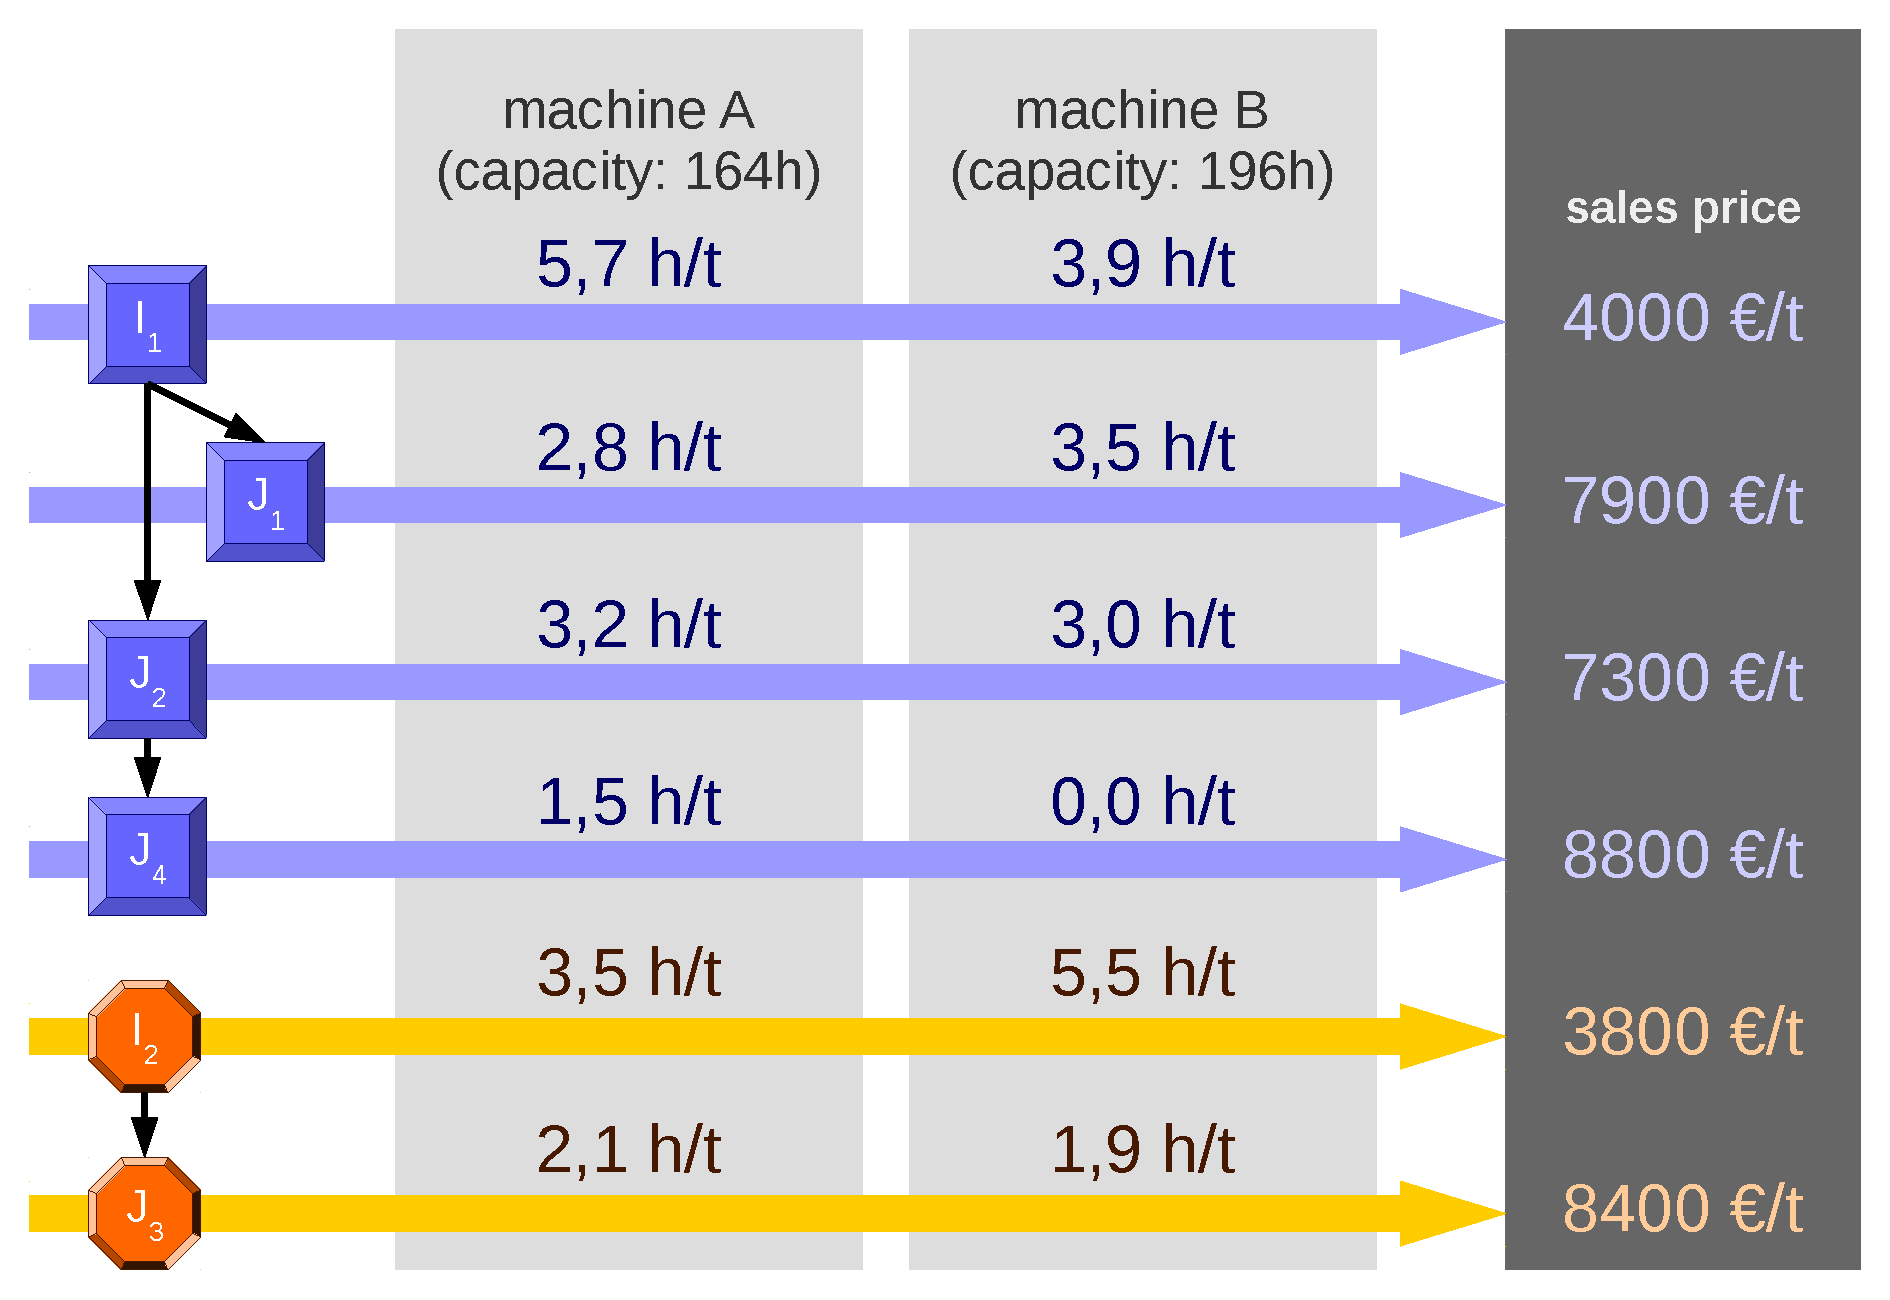
\includegraphics[width=\linewidth]{Bilder/LewigAdelburg}
 \end{figure}
\end{frame}

\begin{frame}
 \frametitle{Concept of a graph: components}
 \begin{center}
  \includegraphics<1>[width=.7\linewidth,page=1]{Bilder/Graph_Lewig_Adelburg}
  \includegraphics<2>[width=.7\linewidth,page=2]{Bilder/Graph_Lewig_Adelburg}
 \end{center}
\end{frame}

\begin{frame}
 \frametitle{Concept of a graph: formal description}
 \begin{itemize}
  \item \textbf{Directed} Graphs are defined as a tuple $G=(V, E)$ with a set of vertices~$V$ and a set of edges~$E\subseteq V\times V$.\\[1ex]
    in example:\\{\footnotesize $G = (\{I_1, I_2, J_1, J_2, J_3, J_4\}, \{(I_1, J_1), (I_1, J_2), (I_2, J_3), (J_2, J_4)\})$}
  \item \textbf{Undirected} graphs are graphs whose edges do not have a specific direction.
  \item \textbf{Weighted} graphs are defined as a tuple $G=(V, E, g)$ with a set of vertices~$V$, a set of edges~$E\subseteq V\times V$ and a weight function $g:E\rightarrow\mathbb{R}$.
 \end{itemize}
\end{frame}
